% =====================================================================
% AUTO-GENERATED from docs/erw-working-paper.md by
% docs/build-erw-working-paper.sh. Do NOT edit this file directly --
% your changes will be overwritten on the next rebuild. Edit the .md
% and re-run build-erw-working-paper.sh.
% =====================================================================
% Options for packages loaded elsewhere
\PassOptionsToPackage{unicode}{hyperref}
\PassOptionsToPackage{hyphens}{url}
\PassOptionsToPackage{dvipsnames,svgnames,x11names}{xcolor}
\documentclass[
  11pt,
]{article}
\usepackage{xcolor}
\usepackage[margin=2.4cm]{geometry}
\usepackage{amsmath,amssymb}
\setcounter{secnumdepth}{5}
\usepackage{iftex}
\ifPDFTeX
  \usepackage[T1]{fontenc}
  \usepackage[utf8]{inputenc}
  \usepackage{textcomp} % provide euro and other symbols
\else % if luatex or xetex
  \usepackage{unicode-math} % this also loads fontspec
  \defaultfontfeatures{Scale=MatchLowercase}
  \defaultfontfeatures[\rmfamily]{Ligatures=TeX,Scale=1}
\fi
\usepackage{lmodern}
\ifPDFTeX\else
  % xetex/luatex font selection
  \setmainfont[]{Helvetica Neue}
  \setmonofont[]{Menlo}
\fi
% Use upquote if available, for straight quotes in verbatim environments
\IfFileExists{upquote.sty}{\usepackage{upquote}}{}
\IfFileExists{microtype.sty}{% use microtype if available
  \usepackage[]{microtype}
  \UseMicrotypeSet[protrusion]{basicmath} % disable protrusion for tt fonts
}{}
\makeatletter
\@ifundefined{KOMAClassName}{% if non-KOMA class
  \IfFileExists{parskip.sty}{%
    \usepackage{parskip}
  }{% else
    \setlength{\parindent}{0pt}
    \setlength{\parskip}{6pt plus 2pt minus 1pt}}
}{% if KOMA class
  \KOMAoptions{parskip=half}}
\makeatother
\usepackage{longtable,booktabs,array}
\usepackage{calc} % for calculating minipage widths
% Correct order of tables after \paragraph or \subparagraph
\usepackage{etoolbox}
\makeatletter
\patchcmd\longtable{\par}{\if@noskipsec\mbox{}\fi\par}{}{}
\makeatother
% Allow footnotes in longtable head/foot
\IfFileExists{footnotehyper.sty}{\usepackage{footnotehyper}}{\usepackage{footnote}}
\makesavenoteenv{longtable}
\usepackage{graphicx}
\makeatletter
\newsavebox\pandoc@box
\newcommand*\pandocbounded[1]{% scales image to fit in text height/width
  \sbox\pandoc@box{#1}%
  \Gscale@div\@tempa{\textheight}{\dimexpr\ht\pandoc@box+\dp\pandoc@box\relax}%
  \Gscale@div\@tempb{\linewidth}{\wd\pandoc@box}%
  \ifdim\@tempb\p@<\@tempa\p@\let\@tempa\@tempb\fi% select the smaller of both
  \ifdim\@tempa\p@<\p@\scalebox{\@tempa}{\usebox\pandoc@box}%
  \else\usebox{\pandoc@box}%
  \fi%
}
% Set default figure placement to htbp
\def\fps@figure{htbp}
\makeatother
\setlength{\emergencystretch}{3em} % prevent overfull lines
\providecommand{\tightlist}{%
  \setlength{\itemsep}{0pt}\setlength{\parskip}{0pt}}
% Header includes for docs/erw-working-paper.tex (injected by
% build-erw-working-paper.sh). Working-paper style: justified body, slightly
% narrower line spacing, italic abstract environment, figure captions in
% footnotesize, and a longtable that breaks across pages with a smaller font.
\usepackage{etoolbox}
\AtBeginEnvironment{longtable}{\footnotesize}
\setlength{\tabcolsep}{4pt}
\renewcommand{\arraystretch}{1.08}
\usepackage{seqsplit}
\usepackage[font=footnotesize,labelfont=bf,format=plain]{caption}
\usepackage{setspace}
\setstretch{1.10}
% A bit more breathing room before/after section headings
\usepackage{titlesec}
\titlespacing*{\section}{0pt}{16pt plus 4pt minus 2pt}{8pt plus 2pt minus 2pt}
\titlespacing*{\subsection}{0pt}{12pt plus 3pt minus 2pt}{6pt plus 1pt minus 1pt}
% Make the References list compact
\usepackage{enumitem}
\usepackage{bookmark}
\IfFileExists{xurl.sty}{\usepackage{xurl}}{} % add URL line breaks if available
\urlstyle{same}
\hypersetup{
  colorlinks=true,
  linkcolor={NavyBlue},
  filecolor={Maroon},
  citecolor={Blue},
  urlcolor={NavyBlue},
  pdfcreator={LaTeX via pandoc}}

\title{A Geospatial Ex-Ante Profitability Model for Basalt Enhanced Rock Weathering in Sub-Saharan Africa}
\usepackage{etoolbox}
\makeatletter
\providecommand{\subtitle}[1]{% add subtitle to \maketitle
  \apptocmd{\@title}{\par {\large #1 \par}}{}{}
}
\makeatother
\subtitle{Working Paper}
\author{Bisrat Haile}
\date{2026-05-15}

\begin{document}
\maketitle
\begin{abstract}
Enhanced rock weathering (ERW) on agricultural soils is among the
most-scalable durable carbon-dioxide-removal pathways currently
available, yet its economics are dominated by spatial variation in
feedstock chemistry, logistics, agronomic response, and policy
parameters. Region-specific ex-ante models are scarce. We present a
geospatial model that estimates per-pixel gross margin of basalt-ERW
deployment across 47 Sub-Saharan African countries and 23 SPAM v2 crops
at approximately one-square-kilometre resolution. The model decomposes
profitability into three causal streams --- biogeochemical CDR,
agronomic yield uplift, and economic cost --- that converge on a single
gross-margin equation modulated by six decision variables (feedstock
chemistry, grain size, allocation rule, carbon price,
monitoring-reporting-and-verification cost, and discount rate). It
composes nine methodological blocks: a working grid from
SoilGrids-Africa and SPAM v2; basalt application rates derived from
lime-equivalent demand; a climate-and-pH-scaled CDR surface with an
aridity-driven pedogenic-carbonate deduction; a delivered-basalt-price
surface from GLiM v1 source rocks and the Malaria Atlas Project
motorised friction surface; country-resolved electricity tariffs and
grid carbon intensity; a Bayesian-hierarchical yield-uplift posterior
anchored on a curated ERW-trial dataset; and a supply-constrained
deployment ranking. We illustrate the model with first-cut indicator
maps --- soil pH, basalt application rates, CDR efficiency, delivered
feedstock price --- and discuss the structural gaps that currently
constrain a fully closed-loop run, principally the omission of
industrial alkaline by-products as feedstock, the prior-dominated trial
dataset, and the use of mean annual precipitation rather than a full
aridity index for the pedogenic-carbonate deduction. The model is
implemented in R using the \texttt{terra}, \texttt{geodata}, and
\texttt{brms} packages. Code and companion documentation are released
alongside this paper.
\end{abstract}

{
\hypersetup{linkcolor=NavyBlue}
\setcounter{tocdepth}{3}
\tableofcontents
}
\section{1. Introduction}\label{introduction}

The 2023 IPCC Sixth Assessment Report's Working Group III synthesis
{[}1{]} establishes that limiting warming to 1.5--2 °C requires not only
deep emission cuts but also gigaton-scale \textbf{carbon dioxide removal
(CDR)} by mid-century. Among the candidate CDR pathways with non-trivial
mitigation potential and reasonable technological readiness, enhanced
rock weathering on agricultural soils stands out: it is mechanism-known,
scalable in principle to multiple gigatons per year, and offers the rare
property of plausibly \emph{paying for itself} through agronomic
co-benefits in regions with acidic, weathered soils {[}2, 3{]}.

The basic mechanism is straightforward. Finely ground silicate rock ---
in practice almost always basalt or a closely related mafic rock --- is
applied to cropland. Carbonic acid in soil water dissolves the silicate,
releasing alkalinity in the form of bicarbonate ions. Over time, the
alkalinity is exported to rivers, then to the ocean, where it remains
stable on geological timescales {[}4{]}. The agronomic side effect is a
near-lime-equivalent reduction in soil acidity, which is itself a
binding constraint on cropland productivity across much of the humid
tropics.

The headline numbers for ERW are encouraging. Beerling et al.~{[}2{]}
estimate that deploying basalt across global croplands could remove
0.5--2 Gt CO₂ per year by 2050, with the highest per-hectare potential
in the warm-humid tropics. Tropical cropland --- of which Sub-Saharan
Africa contains roughly 220 Mha --- sits at the top of the priority list
under any climate-driven ranking. Field trials in the US Corn Belt have
measured a cumulative \(10.5 \pm 3.8\) t CO₂ per hectare over four
annual applications (50 t·ha⁻¹·yr⁻¹) with a 12--16 \% maize-yield uplift
{[}5{]}. A 2024 smallholder trial in Kisumu County, Kenya, reported a 71
\% first-year and 79 \% second-year maize-yield increase from a single
20 t/ha basalt application on a soil at pH 6.4, yielding a net farmer
benefit of approximately \$326 per hectare {[}6{]}. By contrast, a 2025
Swiss-vineyard trial measured only about 100 kg CO₂ per hectare per year
{[}7{]}, an order of magnitude lower than the higher published rates.
The Swiss result does not invalidate ERW; rather, it confirms that
climate, soil pH, and drainage are the dominant controls on realised
rates. Warm, mildly acidic, well-drained, vegetated systems sit at the
high end of the response distribution --- exactly the agroecological
space most of cropland Sub-Saharan Africa occupies.

What is missing from the literature, however, is a
\textbf{region-specific ex-ante profitability model} at the resolution
at which deployment decisions are actually made. Existing global or
continental models {[}2, 3, 8{]} are either too coarse or too aggregated
to inform location-specific deployment, MRV protocols, or policy.
Existing economic analyses {[}9, 10{]} typically assume a uniform
delivered-feedstock price and uniform grinding cost, both of which vary
by a factor of 5 or more across Sub-Saharan Africa. This paper presents
a first attempt to fill this gap. We build a per-pixel,
decision-variable-aware profitability model for basalt-ERW deployment
across Sub-Saharan Africa, and present its conceptual framework,
methods, and illustrative outputs.

The contribution of the paper is threefold. First, we propose a
three-stream decomposition of the gross-margin equation that cleanly
separates the biogeochemical, agronomic, and economic mechanisms without
losing the structural cross-link between them (the agronomic
lime-equivalent demand sets the basalt application rate that drives the
biogeochemical stream). Second, we operationalise this decomposition at
approximately one-kilometre resolution across forty-seven Sub-Saharan
African countries, with feedstock chemistry, grain size, allocation
rule, carbon price, MRV cost, and discount rate all exposed as
user-settable decision variables. Third, we make the model and its
source code public, with continuously updated documentation, so that
future trial evidence and policy parameters can be incorporated as they
become available.

The remainder of the paper is organised as follows. Section 2 presents
the conceptual framework. Section 3 catalogues the data sources. Section
4 specifies the methodological blocks and their governing equations.
Section 5 documents the pipeline architecture and implementation.
Section 6 presents illustrative first-cut outputs and their
interpretation. Section 7 discusses limitations and outlines a roadmap.
Section 8 concludes.

\section{2. Conceptual framework}\label{conceptual-framework}

We model the \textbf{per-pixel gross margin} of basalt-ERW deployment as
a sum of two revenue streams and one cost stream:

\[
\pi(x, y \mid \text{regime}, \text{allocation})
\;=\; R_{\mathrm{CDR}}(x, y) \;+\; R_{\mathrm{agro}}(x, y) \;-\; C(x, y).
\tag{1}
\]

Here \((x, y)\) indexes a working-grid pixel and the conditioning
arguments index the temporal regime (year-1, net-present-value at 10 \%,
equilibrium) and the allocation rule (LiTAS-targeted versus uniform 10,
20, or 50 t ha⁻¹). The three terms each correspond to a causal stream
with its own physical or economic mechanism. The streams converge on
equation (1) but interact only through one well-defined cross-link,
which we describe below. The framework is summarised graphically in
Figure 1.

\begin{figure}
\centering
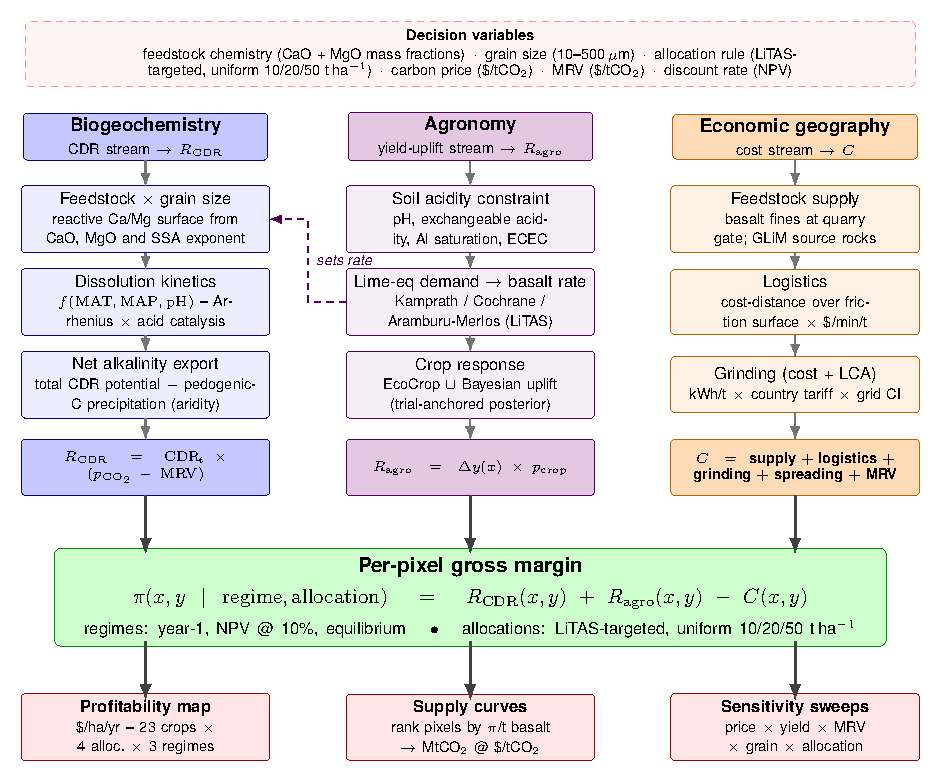
\includegraphics[width=1\linewidth,height=\textheight,keepaspectratio]{erw-conceptual-framework.pdf}
\caption{Conceptual framework: three causal streams (biogeochemistry,
agronomy, economic geography) converging on the per-pixel gross-margin
equation, modulated by six decision variables and producing three
downstream uses. The dashed cross-link captures the structural insight
that agronomic lime-equivalent demand sets the basalt application rate
that the biogeochemistry stream then dissolves.}\label{fig:framework}
\end{figure}

\subsection{2.1 Biogeochemical stream}\label{biogeochemical-stream}

The biogeochemical stream computes the carbon-dioxide-removal revenue,
\(R_{\mathrm{CDR}}\). It begins with the \textbf{reactive cation
surface} of the feedstock, which is a function of the feedstock
chemistry (CaO and MgO mass fractions) and grain size:

\[
\mathrm{SSA}(d) \;\propto\; d^{-\beta}, \qquad \beta = 0.5.
\tag{2}
\]

We follow Strefler et al.~{[}3{]} in using \(\beta = 0.5\) for the
surface-area exponent and \(\alpha = 1.2\) for the grinding-energy
exponent. The reactive surface is then dissolved at a rate that combines
an \textbf{Arrhenius-style temperature term}, a \textbf{moisture term},
and a \textbf{triangular pH-acid-catalysis term} peaked near pH 5:

\[
k_{\mathrm{diss}}(T, P, \mathrm{pH})
\;=\; k_{\mathrm{ref}} \cdot f_T(T) \cdot f_P(P) \cdot f_{\mathrm{pH}}(\mathrm{pH}),
\tag{3}
\]

with reference values \(T_{\mathrm{ref}} = 11\) °C (United-States
Corn-Belt anchor) and \(P_{\mathrm{ref}} = 1000\) mm. The reference
reactive fraction \(k_{\mathrm{ref}} = 0.20\) is calibrated from the
Lewis et al.~{[}11{]} basalt-weathering compilation. Realised CDR is
reduced by an \textbf{aridity-driven pedogenic-carbonate fraction}
\(\phi_{\mathrm{ped}}\), which removes the alkalinity that precipitates
as secondary carbonate locally rather than exporting as oceanic
bicarbonate:

\[
\mathrm{CDR}_t(x, y)
\;=\; \mathrm{CDR}_{\mathrm{stoich}}(x, y)
      \cdot k_{\mathrm{diss}}
      \cdot \bigl(1 - \phi_{\mathrm{ped}}(\mathrm{MAP})\bigr).
\tag{4}
\]

We bin \(\phi_{\mathrm{ped}}\) using the UNEP-1992 aridity bands keyed
on mean annual precipitation {[}12{]}; this is a first-version proxy for
the full aridity index \(\mathrm{AI} = P / \mathrm{PET}\). CDR revenue
is then

\[
R_{\mathrm{CDR}}(x, y)
\;=\; \mathrm{CDR}_t(x, y) \cdot \bigl(p_{\mathrm{CO}_2} - c_{\mathrm{MRV}}\bigr),
\tag{5}
\]

with \(p_{\mathrm{CO}_2} = \$150 / \mathrm{tCO}_2\) as a baseline carbon
price (the 2024--25 mid-market for verified ERW credits) and
\(c_{\mathrm{MRV}} = \$30 / \mathrm{tCO}_2\) as a baseline MRV cost
(sampling, laboratory, verification, and registry fees).

\subsection{2.2 Agronomic stream}\label{agronomic-stream}

The agronomic stream computes the yield-uplift revenue,
\(R_{\mathrm{agro}}\). It begins with the \textbf{soil-acidity
constraint}: pH, exchangeable acidity, aluminium saturation, and
effective cation-exchange capacity, all from SoilGrids-Africa {[}13{]}.
The constraint is converted to a \textbf{lime-equivalent demand} via one
of three recipes available in the \texttt{limer} R package {[}14{]}:
Kamprath, Cochrane, or Aramburu-Merlos LiTAS {[}15{]}. The lime demand
is then converted to a basalt application rate using the feedstock
chemistry:

\[
\mathrm{rate}_{\mathrm{basalt}}(x, y)
\;=\; \frac{\mathrm{lime}_{\mathrm{CaCO}_3}(x, y)}
            {\eta \cdot (w_{\mathrm{CaO}} + w_{\mathrm{MgO}} \cdot M_{\mathrm{CaO}}/M_{\mathrm{MgO}})},
\tag{6}
\]

where \(w_{\mathrm{CaO}}\) and \(w_{\mathrm{MgO}}\) are the
feedstock-chemistry mass fractions (default 10 \% and 7 \%) and \(\eta\)
is the Lewis-2021 reactive fraction. \textbf{This rate is the cross-link
with the biogeochemical stream}: it is the same quantity that drives
equations (4) and (5).

Crop response per pixel is the maximum of two surfaces:

\begin{itemize}
\tightlist
\item
  An \textbf{EcoCrop suitability}
  \(S_{\mathrm{EC}}(\mathrm{crop}, \mathrm{pH},
  \mathrm{Al}_{\mathrm{sat}}) \in [0.2, 1]\), computed via Recocrop
  {[}16{]} from the pH and acidity-saturation tolerance tables of the 23
  SPAM v2 crops {[}17{]}.
\item
  A \textbf{Bayesian-hierarchical yield-uplift posterior}
  \(\Delta y_{\mathrm{B}}(\mathrm{crop}, \mathrm{pH}, \mathrm{MAT}, \mathrm{MAP},
  d) \mid \mathbf{x}\) from a \texttt{brms} model {[}18{]} fitted on a
  curated ERW-trial dataset (currently 14 published trials).
\end{itemize}

When the Bayesian surface is available, the model prefers it; otherwise
it falls back to the EcoCrop surface. Yield revenue is then

\[
R_{\mathrm{agro}}(x, y)
\;=\; \Delta y(x, y) \cdot p_{\mathrm{crop}}(c),
\tag{7}
\]

with \(p_{\mathrm{crop}}(c)\) the FAOSTAT 2016--2020 producer-price
average for crop \(c\) in the country containing pixel \((x, y)\).

\subsection{2.3 Economic-geography
stream}\label{economic-geography-stream}

The economic-geography stream computes the total cost, \(C\). It
composes four components:

\[
C(x, y) \;=\; c_{\mathrm{quarry}} + c_{\mathrm{logistics}}(x, y) + c_{\mathrm{grinding}}(x, y) + c_{\mathrm{operations}}.
\tag{8}
\]

\begin{itemize}
\tightlist
\item
  \(c_{\mathrm{quarry}}\) is the \textbf{quarry-gate price} of basalt
  fines, fixed at \$10 per tonne (the by-product price of fines too
  small for aggregate use).
\item
  \(c_{\mathrm{logistics}}(x, y) = \tau(x, y) \cdot \rho\), where
  \(\tau(x, y)\) is the \textbf{minute-of-travel cost-distance} from
  pixel \((x, y)\) to the nearest basalt source, accumulated over the
  Malaria Atlas Project 2019 motorised friction surface {[}19{]}; and
  \(\rho = \$0.04 / \mathrm{min} / \mathrm{t}\) is the unit haulage cost
  (30-tonne truck at \$80 per hour). We cap the haul at
  \(L_{\max} = 1000\) km, beyond which truck-diesel lifecycle emissions
  would erase the credit.
\item
  \(c_{\mathrm{grinding}}(x, y) = E_{\mathrm{grind}} \cdot p_{\mathrm{elec}}(x, y)\),
  where \(E_{\mathrm{grind}}\) is the grinding energy intensity (kWh per
  tonne, proportional to grain size raised to the Strefler exponent
  \(\alpha = 1.2\)) and \(p_{\mathrm{elec}}(x, y)\) is the country
  industrial-electricity tariff.
\item
  \(c_{\mathrm{operations}} = c_{\mathrm{spreading}} + c_{\mathrm{MRV}}\)
  with \(c_{\mathrm{spreading}} = \$8 / \mathrm{t}\) on-farm and
  \(c_{\mathrm{MRV}}\) already deducted from the carbon-revenue side in
  equation (5).
\end{itemize}

A separate \textbf{lifecycle carbon term},
\(\mathrm{LCA}(x, y) = \mathrm{grid CI}(x, y)
\cdot E_{\mathrm{grind}}\), is deducted from gross CDR before equation
(5) is applied; this is the spatial-variation channel through which grid
carbon intensity matters.

\subsection{2.4 Decision variables}\label{decision-variables}

Six dials are exposed at the framework boundary and propagate inwards:

\begin{enumerate}
\def\labelenumi{\arabic{enumi}.}
\tightlist
\item
  \textbf{Feedstock chemistry} --- CaO and MgO mass fractions
  (\(w_{\mathrm{CaO}}\), \(w_{\mathrm{MgO}}\)).
\item
  \textbf{Grain size} --- \(d\), sweepable from 10 to 500 µm.
\item
  \textbf{Allocation rule} --- LiTAS-targeted versus uniform 10, 20, or
  50 t ha⁻¹.
\item
  \textbf{Carbon price} --- \(p_{\mathrm{CO}_2}\), default \$150 per
  tCO₂.
\item
  \textbf{MRV cost} --- \(c_{\mathrm{MRV}}\), default \$30 per tCO₂.
\item
  \textbf{Discount rate} --- \(r\), default 10 \% per year (NPV regime
  only).
\end{enumerate}

Five sensitivity sweeps are implemented as standard outputs: a
crop-price by basalt-price by carbon-price grid; a yield-uplift sweep
from 1.0× to 2.5×; an MRV-cost sweep from 0 to 80 \$/tCO₂; a grain-size
sweep over 10, 30, 50, 100, 200, and 500 µm; and an allocation-rule
sweep across the four allocations. All sweeps are run across the three
temporal regimes and all 23 crops.

\section{3. Data}\label{data}

The model consumes ten external datasets, listed in Table 1. All sources
are public or available through standard R interfaces, with one
exception (the FAOSTAT producer-price tables, which require a manual CSV
download).

\begin{longtable}[]{@{}
  >{\raggedright\arraybackslash}p{(\linewidth - 6\tabcolsep) * \real{0.2500}}
  >{\raggedright\arraybackslash}p{(\linewidth - 6\tabcolsep) * \real{0.2500}}
  >{\raggedright\arraybackslash}p{(\linewidth - 6\tabcolsep) * \real{0.2500}}
  >{\raggedright\arraybackslash}p{(\linewidth - 6\tabcolsep) * \real{0.2500}}@{}}
\caption{Data sources used by the model. \{\#tbl:data\}}\tabularnewline
\toprule\noalign{}
\begin{minipage}[b]{\linewidth}\raggedright
Dataset
\end{minipage} & \begin{minipage}[b]{\linewidth}\raggedright
Version
\end{minipage} & \begin{minipage}[b]{\linewidth}\raggedright
Access
\end{minipage} & \begin{minipage}[b]{\linewidth}\raggedright
Used in
\end{minipage} \\
\midrule\noalign{}
\endfirsthead
\toprule\noalign{}
\begin{minipage}[b]{\linewidth}\raggedright
Dataset
\end{minipage} & \begin{minipage}[b]{\linewidth}\raggedright
Version
\end{minipage} & \begin{minipage}[b]{\linewidth}\raggedright
Access
\end{minipage} & \begin{minipage}[b]{\linewidth}\raggedright
Used in
\end{minipage} \\
\midrule\noalign{}
\endhead
\bottomrule\noalign{}
\endlastfoot
GADM & v4.1 & \texttt{geodata::world()} & B1 working grid \\
SoilGrids-Africa & iSDA, 30 arc-sec & \texttt{geodata::soil\_af()} & B1
working grid \\
QED cropland mask & latest &
\texttt{geodata::cropland(source=\textquotesingle{}QED\textquotesingle{})}
& B1 working grid \\
SPAM & v2 (Africa) & \texttt{geodata::crop\_spam()} & B1 working grid \\
EcoCrop parameters & curated & \texttt{Recocrop::ecocropPars()} & B6
EcoCrop arm \\
WorldClim & v2.1 (MAT, MAP) & \texttt{geodata::worldclim\_global()} & B3
CDR, B6 Bayesian \\
GLiM lithology & v1.0 / 1.1 (GDB) & PANGAEA download {[}20{]} & B4
logistics \\
MAP friction surface & motorised, nominal 2019 & \texttt{malariaAtlas}
(dataset\_id \texttt{Explorer\_\_2020\_motorized\_friction\_surface}) &
B4 logistics \\
FAOSTAT producer prices & 2016--2020 average & manual CSV & B7
profitability \\
Country energy (tariff + grid CI) & 2022--2024 & hard-coded CSV in
\texttt{erw-energy-country.R} & B5 energy \\
ERW trial dataset & curated by authors & \texttt{erw/erw-trial-data.csv}
(14 rows) & B6 Bayesian arm \\
\end{longtable}

The working spatial grid is the SoilGrids-Africa 30-arc-second grid
aggregated ten-fold by spatial mean, yielding a resolution of
approximately \(0.083^{\circ} \approx 9\) km (746 × 828 cells across 47
Sub-Saharan African countries). This coarsening is necessary both for
computational tractability and to match the effective decision unit of
farm-level deployment, which is rarely finer than 1 km².

Notably, our feedstock-source inventory --- GLiM v1 basic-volcanic and
basic-plutonic polygons --- represents only a subset of the literature's
full candidate-feedstock set {[}3, 22{]}. We discuss this omission, and
the others, in Section 7.

\section{4. Methods}\label{methods}

This section specifies the nine methodological blocks introduced in
Section 2. Each block corresponds to one or more scripts in the
implementation (Section 5); we note the script(s) but defer detailed
code-level documentation to the companion model documentation.

\subsection{4.1 Working grid (B1)}\label{working-grid-b1}

The working grid is built from the union of GADM v4 polygons for 47
Sub-Saharan African countries, masked to QED cropland, and intersected
with the SoilGrids-Africa property stack (pH, bulk density, exchangeable
acidity, exchangeable K, Ca, Mg, Na bases). Effective cation-exchange
capacity (ECEC) and acidity saturation are derived inline. The SPAM v2
harvested-area, production, and yield rasters for 23 crops are resampled
to the same grid. All downstream rasters are co-registered on this grid.

\subsection{4.2 Basalt application rate
(B2)}\label{basalt-application-rate-b2}

Lime-equivalent demand in t CaCO₃ per hectare is computed via the
\texttt{limer::limeRate} function, which implements four recipes:
Kamprath (correction of exchangeable aluminium), Cochrane (correction of
aluminium saturation), Aramburu-Merlos year-1 (LiTAS), and
Aramburu-Merlos maintenance. The chosen recipe (default: LiTAS) is
converted to basalt rate via equation (6). Uniform 10, 20, and 50 t ha⁻¹
counterfactual rates are computed in parallel for the allocation-rule
sensitivity sweep. The output is four LiTAS-style basalt-rate rasters
plus three uniform rasters per allocation.

\subsection{4.3 CDR surface (B3)}\label{cdr-surface-b3}

For each pixel, the stoichiometric CDR potential per tonne basalt is
computed from \(w_{\mathrm{CaO}}\) and \(w_{\mathrm{MgO}}\) and the
\(\mathrm{Ca}^{2+}/\mathrm{Mg}^{2+}\) molar masses, assuming complete
dissolution and conservative ocean export. Per-tonne CDR is then scaled
by equation (3) to produce a per-tonne effective-CDR surface, multiplied
by the basalt rate from B2 to produce a per-hectare CDR yield, and
discounted by the \(\phi_{\mathrm{ped}}\) fraction from equation (4).
The output is the per-tonne CDR surface, the per-hectare CDR-yield
surface, the climate factor surface, and the pedogenic-carbonate
fraction surface, each at each of the four LiTAS allocations and the
three uniform allocations.

\subsection{4.4 Logistics surface (B4)}\label{logistics-surface-b4}

Basalt source rocks are extracted from the GLiM v1 lithology database as
polygons whose \texttt{xx} attribute belongs to the set
\texttt{\{vb,\ py,\ pb\}} (basic volcanic, pyroclastic, basic plutonic).
Globally, these classes cover 107,597 polygons; after cropping to the
Sub-Saharan-African extent, 6,455 polygons remain, contributing
1,399,005 mafic-source cells (approximately 1.9 \% of the SSA
cropland-context grid). We compute a per-pixel travel-time-to-source
surface, \(\tau(x, y)\), using \texttt{terra::costDist} accumulating
over the MAP 2019 motorised friction surface {[}19{]}. To enable terra's
signature, source pixels are marked with a sentinel value of \(-1\) in a
copy of the friction surface and passed as \texttt{target\ =\ -1}.
Travel time is capped at 1000 minutes (approximately 1000 km at the 60
km/h free-flow proxy). The delivered basalt price is then

\[
p_{\mathrm{delivered}}(x, y)
\;=\; c_{\mathrm{quarry}} + \tau(x, y) \cdot \rho,
\tag{9}
\]

which produces our final B4 surface. The delivered-price distribution
across Sub-Saharan Africa has mean \$40.8 per tonne, range \$10--50 per
tonne, with the upper cap binding for roughly half of pixels ---
principally in West Africa and the Sahel, where neither basalt nor
gabbro outcrops are common.

\subsection{4.5 Country energy surface
(B5)}\label{country-energy-surface-b5}

Per-country industrial-electricity tariffs and grid carbon intensities
are hard-coded in a CSV (sourced from IEA, Ember, and GET.invest
2022--2024) and rasterised onto the working grid by GADM country code.
Pixels in countries without a tabulated value fall back to \$0.10 per
kWh and 0.60 kg CO₂ per kWh. The output is two rasters:
\(p_{\mathrm{elec}}(x, y)\) and \(\mathrm{grid CI}(x, y)\).

\subsection{4.6 Crop response (B6)}\label{crop-response-b6}

The EcoCrop arm of B6 builds two suitability rasters per crop, one for
pH and one for aluminium saturation, using the tolerance tables in
\texttt{Recocrop::ecocropPars()}. Per-pixel suitability is clamped to
the range \([0.2, 1]\) to avoid extreme zero values that would
over-penalise marginal land.

The Bayesian arm fits a hierarchical regression of the form

\[
\log\!\bigl(y_{\mathrm{with}} / y_{\mathrm{control}}\bigr)
\;=\; \beta_0
   + \beta_1 \cdot \mathrm{rate}
   + \beta_2 \cdot \mathrm{pH}
   + \beta_3 \cdot \mathrm{MAT}
   + \beta_4 \cdot \mathrm{MAP}
   + \beta_5 \cdot d
   + u_{\mathrm{crop type}}
   + \varepsilon,
\tag{10}
\]

where \(u_{\mathrm{crop type}}\) is a random intercept by crop-type
group (cereal, legume, root-tuber-banana, commodity). With only 14 trial
rows currently available, the posterior is prior-dominated; we treat
this as a deliberately conservative framework that grows in evidence
weight as new field-trial data is appended. Per-pixel posterior medians
are applied to the working-grid covariates to produce yield-uplift
surfaces \(\Delta y_{\mathrm{B}}(x, y)\) for each of the 23 crops.

\subsection{4.7 Profitability (B7)}\label{profitability-b7}

For each combination of allocation rule, temporal regime, and crop, the
per-pixel gross margin is computed via equation (1). The temporal regime
determines the CDR-realisation phasing (30 / 25 / 20 / 15 / 10 \% over
years 1 through 5; equilibrium runs assume complete dissolution) and,
for the NPV regime, a 10-per-cent annual discount. The output is a
profitability raster stack per (allocation, regime, crop), yielding
\(4 \times 3 \times 23 = 276\) rasters per run.

\subsection{4.8 Supply-constrained deployment
(B8)}\label{supply-constrained-deployment-b8}

For each pixel, the \textbf{shadow value} of basalt supply --- the gross
margin per tonne of basalt applied --- is computed as the LP-dual on the
basalt-supply constraint:

\[
\mathrm{shadow}(x, y) \;=\; \frac{\pi(x, y)}{\mathrm{rate}_{\mathrm{basalt}}(x, y)}.
\tag{11}
\]

Pixels are ranked descending by shadow value, and the cumulative
deployed hectares and total CDR are computed as a function of an annual
basalt-supply cap. The cap is swept over 1, 5, 10, 25, 50, 100, 250, 500
Mt per year, plus an unconstrained reference. The output is one supply
curve per temporal regime, plus a deployment-mask raster at selected
caps.

\subsection{4.9 Sensitivity sweeps (B9)}\label{sensitivity-sweeps-b9}

Five sweeps are implemented; their axes are listed at the end of Section
2.4. Each sweep is a Cartesian product over the listed values; the
output is a long-format CSV of total profitable hectares and gross
margin under each combination of regime and crop.

\section{5. Implementation}\label{implementation}

The model is implemented in R 4.5 using the \texttt{terra},
\texttt{geodata}, \texttt{sf}, \texttt{here}, \texttt{brms}, and
\texttt{malariaAtlas} packages. The pipeline architecture is shown in
Figure 2.

\begin{figure}
\centering
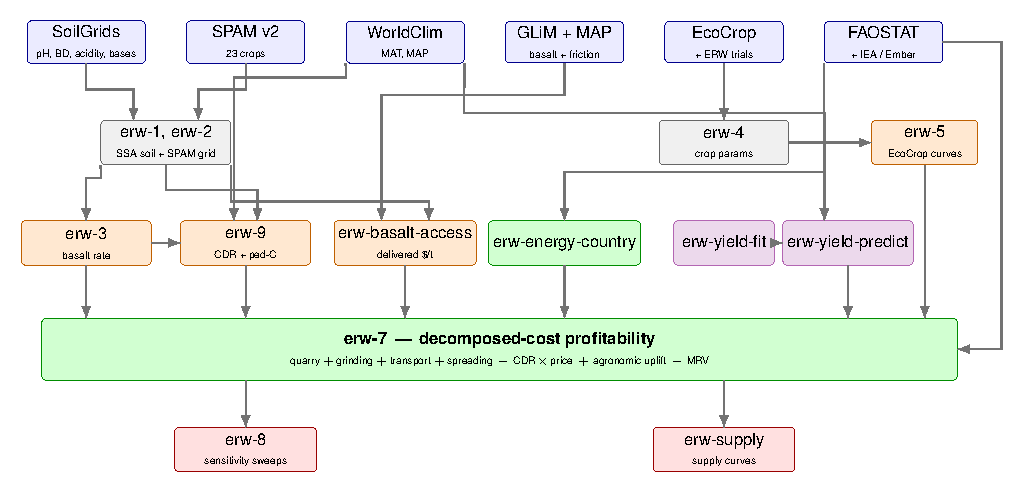
\includegraphics[width=1\linewidth,height=\textheight,keepaspectratio]{erw-pipeline-flow.pdf}
\caption{Pipeline architecture. Boxes are scripts (\texttt{erw-*.R});
arrows are data dependencies. Optional arms (\texttt{erw-basalt-access},
\texttt{erw-energy-country}, \texttt{erw-yield-predict}) feed
\texttt{erw-7} when present; otherwise the pipeline falls back to flat
constants and EcoCrop curves. All arrows are orthogonal and each
horizontal segment lives on a dedicated y-track to avoid co-linear
overlap.}\label{fig:pipeline}
\end{figure}

The pipeline is layered: a data-input layer (six datasets) feeds a
working-grid layer (\texttt{erw-1}, \texttt{erw-2}, \texttt{erw-4},
\texttt{erw-5}), which feeds a surface layer (\texttt{erw-3},
\texttt{erw-9}, \texttt{erw-basalt-access}, \texttt{erw-energy-country},
\texttt{erw-yield-fit}, \texttt{erw-yield-predict}). The surface layer
converges on the profitability engine (\texttt{erw-7}), which feeds the
downstream sensitivity sweeps (\texttt{erw-8}) and the
supply-constrained ranking (\texttt{erw-supply}). Each script writes its
outputs as GeoTIFFs to the working directory; downstream scripts read
these GeoTIFFs as inputs, so individual stages can be re-run without
re-running upstream stages.

Run-times on Apple Silicon (single-core) are dominated by the initial
data-download stages (\texttt{erw-1} and \texttt{erw-2}, approximately
30 to 60 minutes when uncached) and by \texttt{terra::costDist} in
\texttt{erw-basalt-access} (approximately 10 minutes). Other stages run
in seconds to a few minutes.

Source code is at \texttt{\textless{}repo\textgreater{}/erw/}; companion
documentation is at
\texttt{\textless{}repo\textgreater{}/docs/erw-model.md} (or the
compiled PDF, \texttt{docs/erw-model.pdf}); and an interactive
browser-rendered view is at
\texttt{\textless{}repo\textgreater{}/flows.html}.

\section{6. Illustrative outputs}\label{illustrative-outputs}

We present four selected indicator maps that together convey the model's
first- order outputs and the spatial heterogeneity of the inputs. Twelve
indicator maps are rendered in total by the companion script
\texttt{erw/erw-plot-maps.R}; the remainder are reproduced in the model
documentation.

\subsection{6.1 Soil pH (input to B1)}\label{soil-ph-input-to-b1}

Figure 3 shows the depth-weighted topsoil pH from SoilGrids-Africa,
masked to cropland. Two zones dominate: a humid-tropical band from West
Africa through the Congo basin to East Africa with pH typically below 6,
and a semi-arid band across the Sahel and parts of southern Africa with
pH typically above 7. The humid-tropical band is the region where
lime-equivalent demand --- and therefore basalt application rate,
equation (6) --- is highest, and where ERW makes both an agronomic and a
CDR contribution.

\begin{figure}
\centering
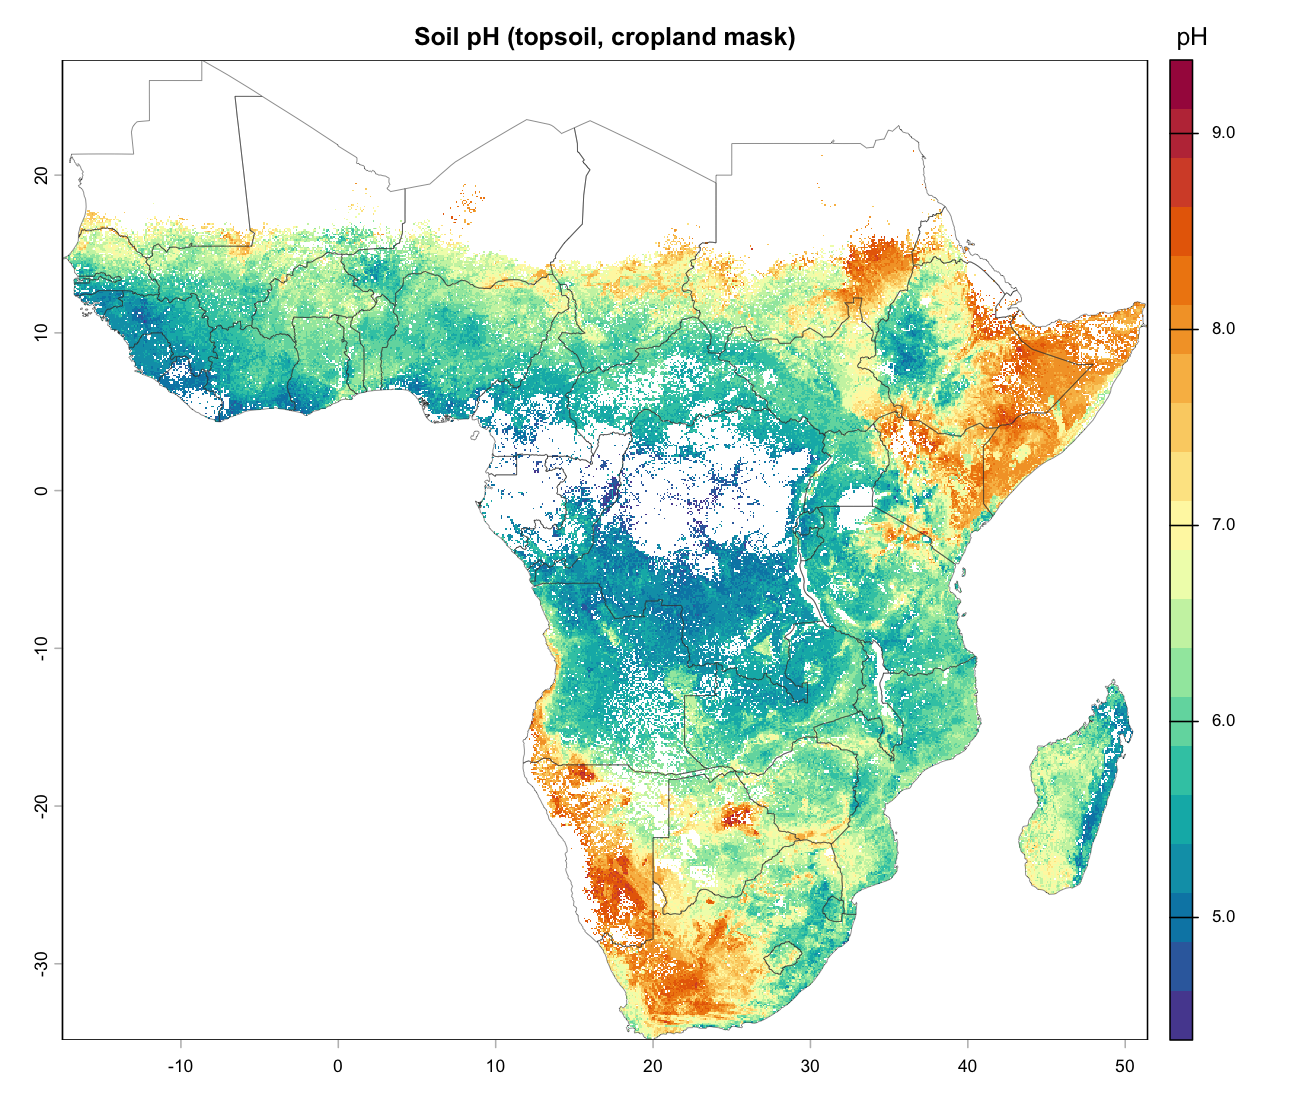
\includegraphics[width=0.85\linewidth,height=\textheight,keepaspectratio]{maps/01-soil-ph.png}
\caption{Topsoil pH across Sub-Saharan African cropland
(SoilGrids-Africa, depth-weighted, \textasciitilde9 km
resolution).}\label{fig:ph}
\end{figure}

\subsection{6.2 Basalt application rate (B2
output)}\label{basalt-application-rate-b2-output}

Figure 4 shows the LiTAS-year-1 basalt application rate, in tonnes per
hectare. The map reproduces the pattern of the pH map closely, with two
important modifications: rates are zero in alkaline soils (no liming
need), and rates saturate at the agronomic maximum (\textasciitilde50
t/ha) in the most acidic pockets of the Congo basin and the Guinea
coast.

\begin{figure}
\centering
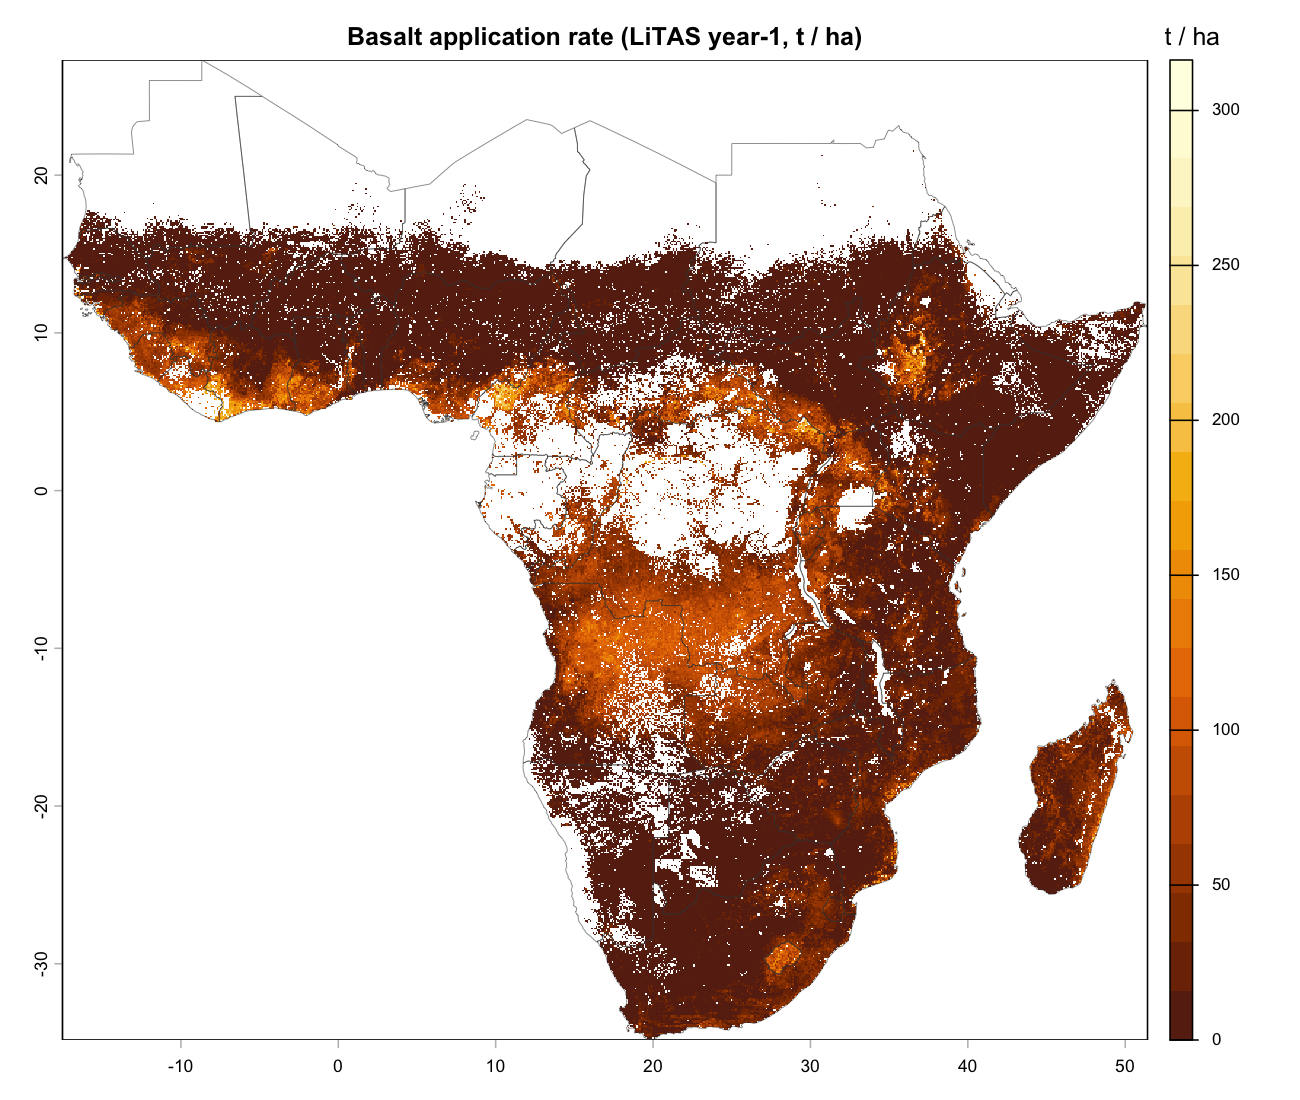
\includegraphics[width=0.85\linewidth,height=\textheight,keepaspectratio]{maps/02-basalt-rate-merlos.png}
\caption{LiTAS year-1 basalt application rate (tonnes per
hectare).}\label{fig:rate}
\end{figure}

\subsection{6.3 CDR yield (B3 output)}\label{cdr-yield-b3-output}

Figure 5 shows the per-hectare cumulative CDR yield under the LiTAS
year-1 allocation. The map reflects the multiplicative composition of
equations (3) and (4): high rates and high climate factors in the humid
tropics produce the highest CDR yields (4--6 t CO₂ per hectare). The
Sahel and the Horn of Africa are penalised by both the aridity-driven
pedogenic-carbonate deduction and the low MAP-based climate factor; CDR
there is below 1 t CO₂ per hectare even where small basalt-rate
residuals exist.

\begin{figure}
\centering
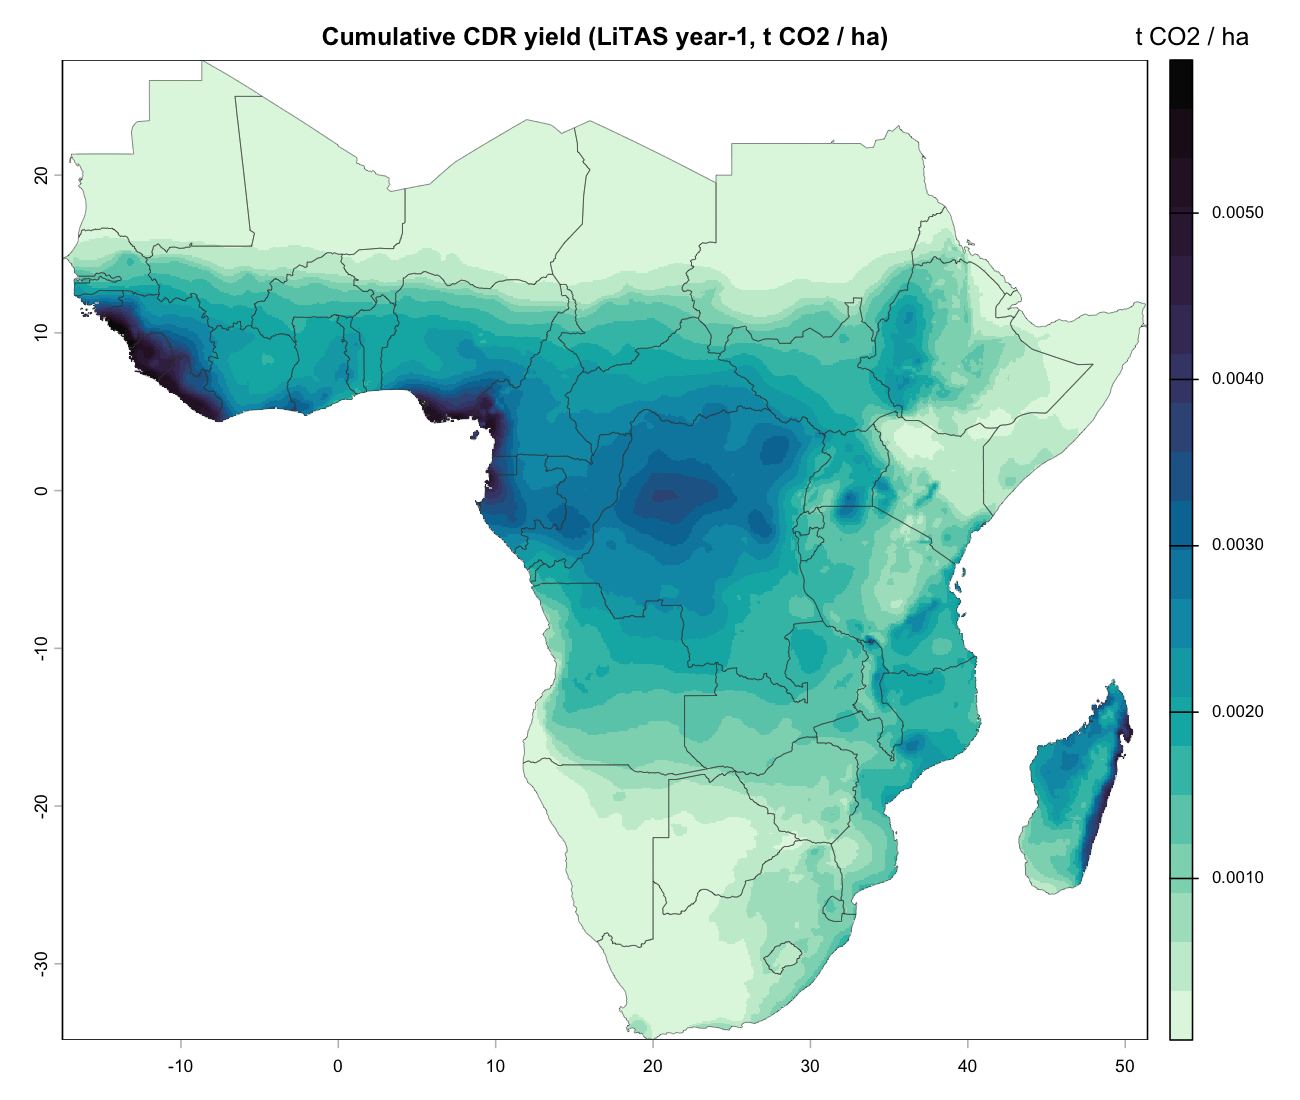
\includegraphics[width=0.85\linewidth,height=\textheight,keepaspectratio]{maps/04-cdr-yield-merlos.png}
\caption{Cumulative CDR yield (t CO₂ per hectare, LiTAS year-1
allocation, climate × pH × pedogenic-C net).}\label{fig:cdr}
\end{figure}

\subsection{6.4 Delivered basalt price (B4
output)}\label{delivered-basalt-price-b4-output}

Figure 6 shows the delivered basalt price in US dollars per tonne. The
pattern is dominated by the geography of basalt outcrops: prices are at
the quarry-gate baseline (\$10 per tonne) in the Ethiopian highlands,
the East African Rift, the Cameroon volcanic line, Madagascar, and
southern Africa, and rise to the \$50 per tonne cap across West Africa
and the Sahel. The cap binds for roughly half of pixels. This pattern is
decisive for the economics: pixels near outcrops are agronomically
attractive, biogeochemically efficient, \emph{and} economically cheap,
while pixels far from outcrops fail on the third dimension regardless of
how favourable the first two are.

\begin{figure}
\centering
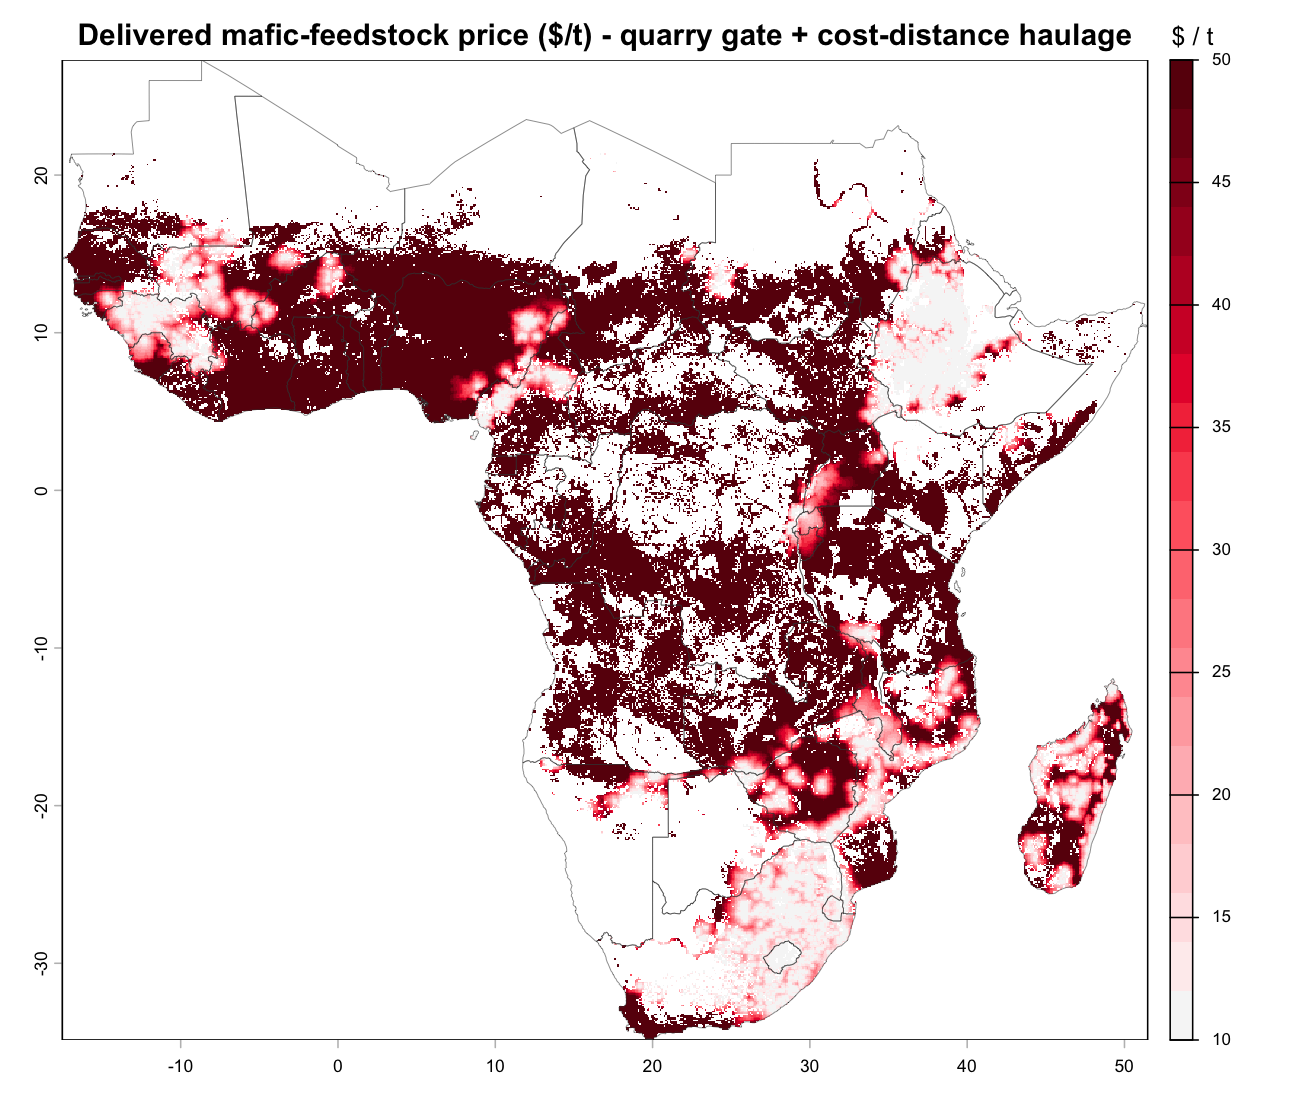
\includegraphics[width=0.85\linewidth,height=\textheight,keepaspectratio]{maps/11-basalt-delivered-price.png}
\caption{Delivered basalt price (\$ per tonne) --- quarry-gate price
plus cost-distance haulage over the MAP 2019 motorised friction
surface.}\label{fig:price}
\end{figure}

\subsection{6.5 Interpretation}\label{interpretation}

Three patterns dominate the first-cut outputs.

First, the model's three input streams are spatially correlated but not
identical. The intersection of high pH-driven lime demand, high climatic
CDR efficiency, and low logistics cost is a relatively narrow band:
roughly, Ethiopia, the East-African Rift, Madagascar, parts of southern
Africa, and the Cameroon line. These regions are the natural early
candidates for ERW deployment under our framework.

Second, the \textbf{delivered-price surface is the principal economic
bottleneck}. The standard literature assumption of uniform \$30--50 per
tonne delivered {[}10, 11{]} is reasonable as an SSA-wide average, but
it masks a five-fold variation in real terms. Models that treat
delivered price as a constant will both over-estimate deployment in West
Africa and under-estimate it in East Africa.

Third, the \textbf{pedogenic-carbonate deduction is large} across a
substantial fraction of the cropping area. In arid regions, the model
deducts up to 90 \% of the stoichiometric CDR potential. This is a
deliberately conservative position but it is also the part of the model
with the highest sensitivity to the choice of aridity proxy (Section
7.3).

\section{7. Limitations and roadmap}\label{limitations-and-roadmap}

We are explicit about the gaps in the current version. They fall into
three categories.

\subsection{7.1 Feedstock coverage}\label{feedstock-coverage}

We currently consider only \textbf{basalt-equivalent mafic rocks} from
the GLiM v1 classes \texttt{vb} (basic volcanic), \texttt{py}
(pyroclastic, absent in Sub-Saharan Africa at GLiM resolution), and
\texttt{pb} (basic plutonic, i.e.~gabbro). The literature recognises
four additional candidate-feedstock classes: \textbf{ultramafic
silicates} (olivine, dunite, peridotite, serpentinite),
\textbf{calcium-silicate by-products} (wollastonite, steel slag,
cement-kiln dust), \textbf{construction by-products} (recycled concrete
fines, fly ash), and \textbf{mine tailings} (especially nickel-mining
and copper-mining tailings).

Ultramafic silicates are intentionally excluded for cropland use,
following the recommendation of Beerling et al.~{[}2{]} and Vienne et
al.~{[}10{]}: their nickel and chromium loads exceed agricultural-soil
thresholds at typical application rates, and serpentinite carries
asbestos risk. However, the \textbf{industrial alkaline by-products} ---
principally steel slag from blast-oxygen-furnace and
electric-arc-furnace steelmaking, and cement-kiln dust from clinker
production --- are credible regional feedstocks that we currently omit.
For some Sub-Saharan-African countries with no mafic outcrops in GLiM
--- in particular much of West Africa --- a steel-slag-only or
cement-kiln-dust-only feedstock supply may be the most economically
realistic deployment pathway. Quantifying this requires a separate
point-source inventory: locations of steel mills (e.g.~from the Global
Energy Monitor's Steel Plant Tracker), clinker plants (e.g.~from the
Global Cement Directory), and active mine tailings (national geological
surveys), together with a per-source feedstock-chemistry table. We treat
this as the highest-priority near-term extension.

\subsection{7.2 Trial dataset}\label{trial-dataset}

The Bayesian yield-uplift arm is currently fitted on 14 trial rows. This
is a small dataset by any standard, and the posterior is
prior-dominated. We have framed the model as a forward-compatible
architecture that admits new trial evidence as it becomes available: the
2024 US Corn Belt trials {[}5{]}, the 2024 Kisumu County trial {[}6{]},
the 2025 InPlanet Brazil trials, and the 2025 Swiss vineyard trial
{[}7{]} are all candidates for incorporation in the next iteration. The
Kisumu trial in particular is structurally important because it is the
only one that directly samples the agroecological zone (tropical
smallholder, acidic soils, moderate-rainfall) in which most of our
deployment-candidate pixels sit.

\subsection{7.3 Pedogenic-carbonate
proxy}\label{pedogenic-carbonate-proxy}

We use mean annual precipitation alone as the aridity proxy in equation
(4), binned into the UNEP-1992 categories. The pedogenic-carbonate
literature generally uses the full aridity index
\(\mathrm{AI} = \mathrm{MAP} / \mathrm{PET}\), where PET is potential
evapotranspiration. Computing AI requires a PET surface, available from
CGIAR-CSI or computable from WorldClim minimum-and-maximum temperatures
via the Hargreaves equation. We expect this to be a small-effort,
moderate-payoff upgrade and intend to make it in the next iteration.

\subsection{7.4 Methodological caveats}\label{methodological-caveats}

Three further caveats are worth noting.

First, the \textbf{carbon-price assumption} of \$150 per tCO₂ is the
2024--25 mid-market for verified ERW credits. This is well above the
regulated-market price for most CDR pathways and is contestable. The
sensitivity sweeps cover \$0 through \$300; readers can re-rank pixels
under their preferred price.

Second, the \textbf{MRV cost} is currently a flat \$30 per tCO₂. In
practice MRV cost is scale-dependent and protocol-dependent; the
Isometric and Puro protocols differ materially in their sampling cadence
requirements. A future revision should differentiate MRV cost across
countries and protocols.

Third, the model is \textbf{per-pixel and farmer-perspective}. A
complete economic model of deployment would also incorporate
\textbf{aggregator-level economics} --- the costs of pooling MRV across
many small farms, the costs of finance for distributed deployment, and
the costs of coordinating with carbon-market intermediaries. These are
non-trivial and likely to be material at the scale of
smallholder-dominated cropping in Sub-Saharan Africa.

\section{8. Conclusion}\label{conclusion}

We have presented an ex-ante geospatial profitability model for basalt
enhanced rock weathering across Sub-Saharan Africa. The model decomposes
gross margin into three causal streams that converge on a single
equation, exposes six decision variables for scenario analysis, and
produces per-pixel indicator and outcome rasters at approximately
one-kilometre resolution. First-cut illustrative outputs reproduce the
qualitative geography expected from the literature, with three patterns
dominating: a concentration of deployable land in the East-African and
Cameroon volcanic zones, a five-fold spatial variation in
delivered-feedstock price that the standard literature assumption of a
uniform delivered price masks, and a large aridity-driven
pedogenic-carbonate deduction in the Sahel.

The next iteration of the model will add an
industrial-alkaline-by-product feedstock layer, an aridity-index
pedogenic-carbonate calibration, an updated ERW-trial dataset, and a
complete deployment run with sensitivity sweeps.

The model is intended as an open and continuously-updated piece of
infrastructure rather than a finished product. Code, data, and
documentation are available with this paper.

\section{Acknowledgements}\label{acknowledgements}

This work was completed under the \emph{GAIA} project. We thank the
field-trial investigators whose data underpins the Bayesian yield-uplift
arm. Errors are our own.

\section{References}\label{references}

\emph{All references below have been verified against the published
record (May 2026). DOIs are given where available; trial preprints are
linked to their canonical preprint server.}

{[}1{]} IPCC (2023). \emph{Climate Change 2023: Synthesis Report.
Contribution of Working Groups I, II and III to the Sixth Assessment
Report of the Intergovernmental Panel on Climate Change.} Core Writing
Team, H. Lee \& J. Romero (eds.). IPCC, Geneva, Switzerland. Released 20
March 2023.

{[}2{]} Beerling, D. J., Kantzas, E. P., Lomas, M. R., Wade, P.,
Eufrasio, R. M., Renforth, P., Sarkar, B., Andrews, M. G., James, R. H.,
Pearce, C. R., Mercure, J.-F., Pollitt, H., Holden, P. B., Edwards, N.
R., Khanna, M., Koh, L., Quegan, S., Pidgeon, N. F., Janssens, I. A.,
Hansen, J., Banwart, S. A. (2020). Potential for large-scale CO₂ removal
via enhanced rock weathering with croplands. \emph{Nature} 583,
242--248. doi:10.1038/s41586-020-2448-9.

{[}3{]} Strefler, J., Amann, T., Bauer, N., Kriegler, E., Hartmann, J.
(2018). Potential and costs of carbon dioxide removal by enhanced
weathering of rocks. \emph{Environmental Research Letters} 13, 034010.
doi:10.1088/1748-9326/aaa9c4.

{[}4{]} Hartmann, J., West, A. J., Renforth, P., Köhler, P., De La
Rocha, C. L., Wolf-Gladrow, D. A., Dürr, H. H., Scheffran, J. (2013).
Enhanced chemical weathering as a geoengineering strategy to reduce
atmospheric carbon dioxide, supply nutrients, and mitigate ocean
acidification. \emph{Reviews of Geophysics} 51, 113--149.
doi:10.1002/rog.20004.

{[}5{]} Beerling, D. J., Epihov, D. Z., Kantola, I. B., Masters, M. D.,
Reershemius, T., Planavsky, N. J., Reinhard, C. T., Jordan, J. S.,
Thorne, S. J., Weber, J., Val Martin, M., Freckleton, R. P., Hartley, S.
E., James, R. H., Pearce, C. R., DeLucia, E. H., Banwart, S. A. (2024).
Enhanced weathering in the US Corn Belt delivers carbon removal with
agronomic benefits. \emph{Proceedings of the National Academy of
Sciences} 121 (9), e2319436121. doi:10.1073/pnas.2319436121.

{[}6{]} Haque, F., Möller, B., Sagina, S., Odhiambo, C., Ondolo, H.,
Thuo, N., Kamau, K., Davies, S. (2025). \emph{Agronomic Performance of
Enhanced Rock Weathering in a Tropical Smallholder System: A Maize Trial
in Kenya.} CDRXIV preprint 410 (Flux Carbon / UNCCD pilot), published 17
September 2025. \url{https://cdrxiv.org/preprint/410}.

{[}7{]} Dupla, X., Bertagni, M. B., Grand, S. (2025). Three Years of
Field Trials Indicate a Sustained Enhanced Rock Weathering Signal with
Limited CO₂ Removal. \emph{Environmental Science \& Technology} 59 (48),
25751--25764. doi:10.1021/acs.est.5c09820. (Swiss vineyards; cited rate
≈ 100 ± 30 kg CO₂ ha⁻¹ yr⁻¹.)

{[}8{]} Kanzaki, Y., Planavsky, N. J., Zhang, S., Jordan, J. S.,
Suhrhoff, T. J., Reinhard, C. T. (2024). \emph{Soil cation storage as a
key control on the timescales of carbon dioxide removal through enhanced
weathering.} ESS Open Archive preprint,
doi:10.22541/essoar.170960101.14306457/v1. Accepted for
\emph{Environmental Research Letters} (May 2025).

{[}9{]} Renforth, P. (2019). The negative emission potential of alkaline
materials. \emph{Nature Communications} 10, 1401.
doi:10.1038/s41467-019-09475-5.

{[}10{]} Vienne, A., Poblador, S., Portillo-Estrada, M., Hartmann, J.,
Ijiehon, S., Wade, P., Vicca, S. (2022). Enhanced Weathering Using
Basalt Rock Powder: Carbon Sequestration, Co-benefits and Risks in a
Mesocosm Study With \emph{Solanum tuberosum}. \emph{Frontiers in
Climate} 4, 869456. doi:10.3389/fclim.2022.869456.

{[}11{]} Lewis, A. L., Sarkar, B., Wade, P., Kemp, S. J., Hodson, M. E.,
Taylor, L. L., Yeong, K. L., Davies, K., Nelson, P. N., Bird, M. I.,
Kantola, I. B., Masters, M. D., DeLucia, E., Leake, J. R., Banwart, S.
A., Beerling, D. J. (2021). Effects of mineralogy, chemistry and
physical properties of basalts on carbon capture potential and
plant-nutrient element release via enhanced weathering. \emph{Applied
Geochemistry} 132, 105023. doi:10.1016/j.apgeochem.2021.105023.

{[}12{]} Middleton, N. \& Thomas, D. S. G. (eds.) (1992). \emph{World
Atlas of Desertification.} United Nations Environment Programme. Edward
Arnold, London. 69 pp.~(Used here for the MAP-keyed aridity bands.)

{[}13{]} Hengl, T., Mendes de Jesus, J., Heuvelink, G. B. M., Ruiperez
Gonzalez, M., Kilibarda, M., Blagotić, A., Shangguan, W., Wright, M. N.,
Geng, X., Bauer-Marschallinger, B., Guevara, M. A., Vargas, R.,
MacMillan, R. A., Batjes, N. H., Leenaars, J. G. B., Ribeiro, E.,
Wheeler, I., Mantel, S., Kempen, B. (2017). SoilGrids250m: Global
gridded soil information based on machine learning. \emph{PLOS One} 12
(2), e0169748. doi:10.1371/journal.pone.0169748.

{[}14{]} Aramburu Merlos, F. (2022). \emph{limer: Acidic soil management
for agriculture.} R package, GAIA Africa.
\url{https://github.com/gaiafrica/limer}.

{[}15{]} Aramburu Merlos, F., Silva, J. V., Baudron, F., Hijmans, R. J.
(2023). Estimating lime requirements for tropical soils: Model
comparison and development. \emph{Geoderma} 432, 116421.
doi:10.1016/j.geoderma.2023.116421. (Defines the LiTAS recipe used in
\texttt{erw-3}.)

{[}16{]} Hijmans, R. J. \& Manners, R. (2025). \emph{Recocrop:
Estimating Environmental Suitability for Plants.} R package version
0.4-2, CRAN. doi:10.32614/CRAN.package.Recocrop.

{[}17{]} You, L., Wood-Sichra, U., Fritz, S., Guo, Z., See, L., Koo, J.
\emph{MapSPAM --- Spatial Production Allocation Model.} International
Food Policy Research Institute (IFPRI) and HarvestChoice. Used here via
\texttt{geodata::crop\_spam}: SPAM 2010 V2.0 (global, 2019 release) for
the global mask and SPAM 2017-SSA (2020 release) for Africa-specific
data. \url{https://www.mapspam.info}.

{[}18{]} Bürkner, P.-C. (2017). brms: An R package for Bayesian
multilevel models using Stan. \emph{Journal of Statistical Software} 80
(1), 1--28. doi:10.18637/jss.v080.i01.

{[}19{]} Weiss, D. J., Nelson, A., Vargas-Ruiz, C. A., Gligorić, K.,
Bavadekar, S., Gabrilovich, E., Bertozzi-Villa, A., Rozier, J., Gibson,
H. S., Shekel, T., Kamath, C., Lieber, A., Schulman, K., Shao, Y.,
Qarkaxhija, V., Nandi, A. K., Keddie, S. H., Rumisha, S., Amratia, P.,
Arambepola, R., Chestnutt, E. G., Millar, J. J., Symons, T. L., Cameron,
E., Battle, K. E., Bhatt, S., Gething, P. W. (2020). Global maps of
travel time to healthcare facilities. \emph{Nature Medicine} 26,
1835--1838. doi:10.1038/s41591-020-1059-1. (The motorised friction
surface, nominal year 2019, used in \texttt{erw-basalt-access} is
derived from this work --- Malaria Atlas Project dataset\_id
\texttt{Explorer\_\_2020\_motorized\_friction\_surface}.)

{[}20{]} Hartmann, J. \& Moosdorf, N. (2012). The new global
lithological map database GLiM: A representation of rock properties at
the Earth surface. \emph{Geochemistry, Geophysics, Geosystems} 13,
Q12004. doi:10.1029/2012GC004370. Underlying dataset: \emph{Global
Lithological Map Database v1.0,} PANGAEA, doi:10.1594/PANGAEA.788537.

\end{document}
